  \begin{figure}[H]
\begin{center}
    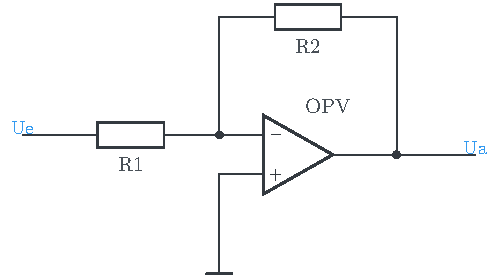
\includegraphics[width=0.618\textwidth]{circuits/inv_verst.pdf}
\end{center}
    \caption{Invertierende Verstärkerschaltung}
  \end{figure}

\begin{gather*}
  U_a = V_0(U_p-U_n)\\
  U_p = 0 \, \si{\volt}\\
  U_a = -V_0 \cdot U_n\\
  \intertext{Bestimmung von $U_n$ durch Überlagerung der Eingangs- und
    Ausgangswirkung:}
  U_n = U_n' + U_n''\\
  U_n' = U_n|_{U_a=0}\\
  = U_e \cdot \frac{R_2}{R_1 + R_2}\\
  U_n'' = U_n|_{U_e=0}\\
  = U_a \cdot \frac{R_1}{R_1 + R_2}\\
  U_a = -V_0 \cdot U_e \cdot \frac{R_2}{R_1+R_2} - V_0 \cdot U_a \cdot
  \frac{R_1}{R_1+R_2}\\
  U_a (1 + V_0 \cdot \frac{R_1}{R_1+R_2}) = -V_0 \cdot U_e \cdot \frac{R_2}{R_1+R_2}\\
  \frac{U_a}{U_e} = V = - \frac{V_0 \cdot \frac{R_2}{R_1+R_2}}{1+V_0 \cdot
    \frac{R_1}{R_1+R_2}} = - \frac{V_0}{(R_1+R_2) + V_0 \cdot R_1}\\
  V = - \frac{R_2}{\frac{R_1+R_2}{V_0} + R_1}\\
  \intertext{für $V_0 \rightarrow \infty$}
  V = -\frac{R_2}{R_1}
\end{gather*}